% %******************************************************************************
% % % sistema.tex % teste web
% %******************************************************************************
% % % Title......: Sistema proposto % % Author.....: GSCAR-DFKI % % Started....:
% Nov 2013 % % Emails.....: renan028@gmail.com % % Address....: Universidade
% Federal do Rio de Janeiro %              Caixa Postal 68.504, CEP: 21.945-970
% %              Rio de Janeiro, RJ - Brasil.
% %
% %******************************************************************************


% %******************************************************************************
% % SECTION - Sistema proposto
% %******************************************************************************
\section{Sistema proposto}
O objetivo do projeto ROSA é entregar uma solução para monitoramento, inspeção e
remoção de sedimentos, de forma que as falhas comentadas nas seções anteriores
sejam minimizadas e as operações sejam mais seguras. Esta seção é subdividida em
uma descrição geral de dispositivos que compõem o projeto e nos modos de
operações excepcionais expostos em seções anteriores.

% %******************************************************************************
% % SUBSECTION - Subsection
% %******************************************************************************


\subsection{Operação padrão (inspeção e remoção)}
A principal preocupação do operador nas operações padrões se resume ao encaixe
bem sucedido entre garra e stoplog. Este encaixe deve ser constantemente
monitorado, tornando-se necessária a instrumentação do Lifting Beam. O sistema
será composto por sensores, eletrônica embarcada, sinalizadores e eletrônica da
base, e um carretel com umbilical, responsável pelo fornecimento de energia e
interface de comunicação entre base e eletrônica embarcada (FIGURA).

\subsubsection{Sensores}
O sistema é composto pelos dispositivos:
\begin{itemize}
\item Dois encoders absolutos.
\item Dois sensores indutivos de proximidade.
\item Sensor de inclinação.
\item Sensor de profundidade.
\end{itemize}

Os encoders serão acoplados ao eixo de rotação da garra pescadora. O
monitoramento do deslocamento angular das garras independentemente torna
possível a identificação de falhas de encaixe. Durante a operação de encaixe, o
eixo da garra percorre ângulos já conhecidos: o ângulo sofre leve abertura e
volta a $90^o$ no encaixe. 

Os sensores indutivos de proximidade serão instalados na garra pescadora,
próximo ao local de contato com o stoplog. Indicarão o acoplamento das garras
com o stoplog, a partir da geração de campo magnético. Esses sensores só serão
excitados em casos de proximidade com metais, sendo possível assim a
identificação de obstáculos no encaixe do stoplog. 

O sensor de inclinação ficará localizado junto à eletrônica embarcada, na parte
central do Lifting Beam. O monitoramento da inclinação do Lifting Beam é
importante na identificação de encaixe mal sucedido ou danos no equipamento. O
sensor será do tipo capacitivo.

O sensor de profundidade também ficará localizado junto à eletrônica embarcada,
na parte central do Lifting Beam. O sensor trabalha com diferença de pressão e
será importante na identificação da localização do Lifting Beam quando submerso.

\subsubsection{Eletrônica embarcada}
A eletrônica embarcada é composta por: 

\begin{itemize}
	\item PC embarcado industrial com ethernet, RS485 e interface CAN
	\item  conversores DC/DC
	\item  placa microcontroladora com sensor de inclinação, sensor de profundidade, sensor de ingresso 	 	e portas para 2 sensores analógicos. 
	\item circuito supervisório
\end{itemize}

A eletrônica embarcada terá encapsulamento à  água,
choque e resistente mínima de 5 bar de pressão. O encapsulamento deve possuir 8 connectores subconn a prova d'agua para conectar os equipamentos externos: 

\begin{itemize}
 	\item um Super Seaking Profiler DFP from Tritech
 	\item um Gemini 720i from Tritech
	\item um Micron Sonar DST 750m from Tritech
	\item um OE10-10 from Kongsberg
	\item dois NBB20-L2-E2-V1 from Pepperl-Fuchs
	\item dois RM9000 from IFM 
\end{itemize}



O circuito supervisório será responsável por distribuir a alimentação aos
dispositivos, monitorar essa potência fornecida e proteger os equipamentos
contra sobrecorrente/voltagem. Será composta por relés, microcontroladores e
outros componentes eletrônicos.

Conversores DC/DC realizam o condicionamento do sinal. Os dispositivos têm
alimentação variada e o umbilical fornece apenas um nível de tensão, dessa forma
há a necessidade de conversores para distribuírem a potência como requerida
entre os dispositivos.

A eletrônica embarcada será conectada a uma eletrônica de terra por um umbilical e operará submersa. 

O diagrama~\ref{EE_1} mostra as interfaces de comunicação da eletrônica proposta
para esta solução.

\begin{figure}[H]
    \centering
    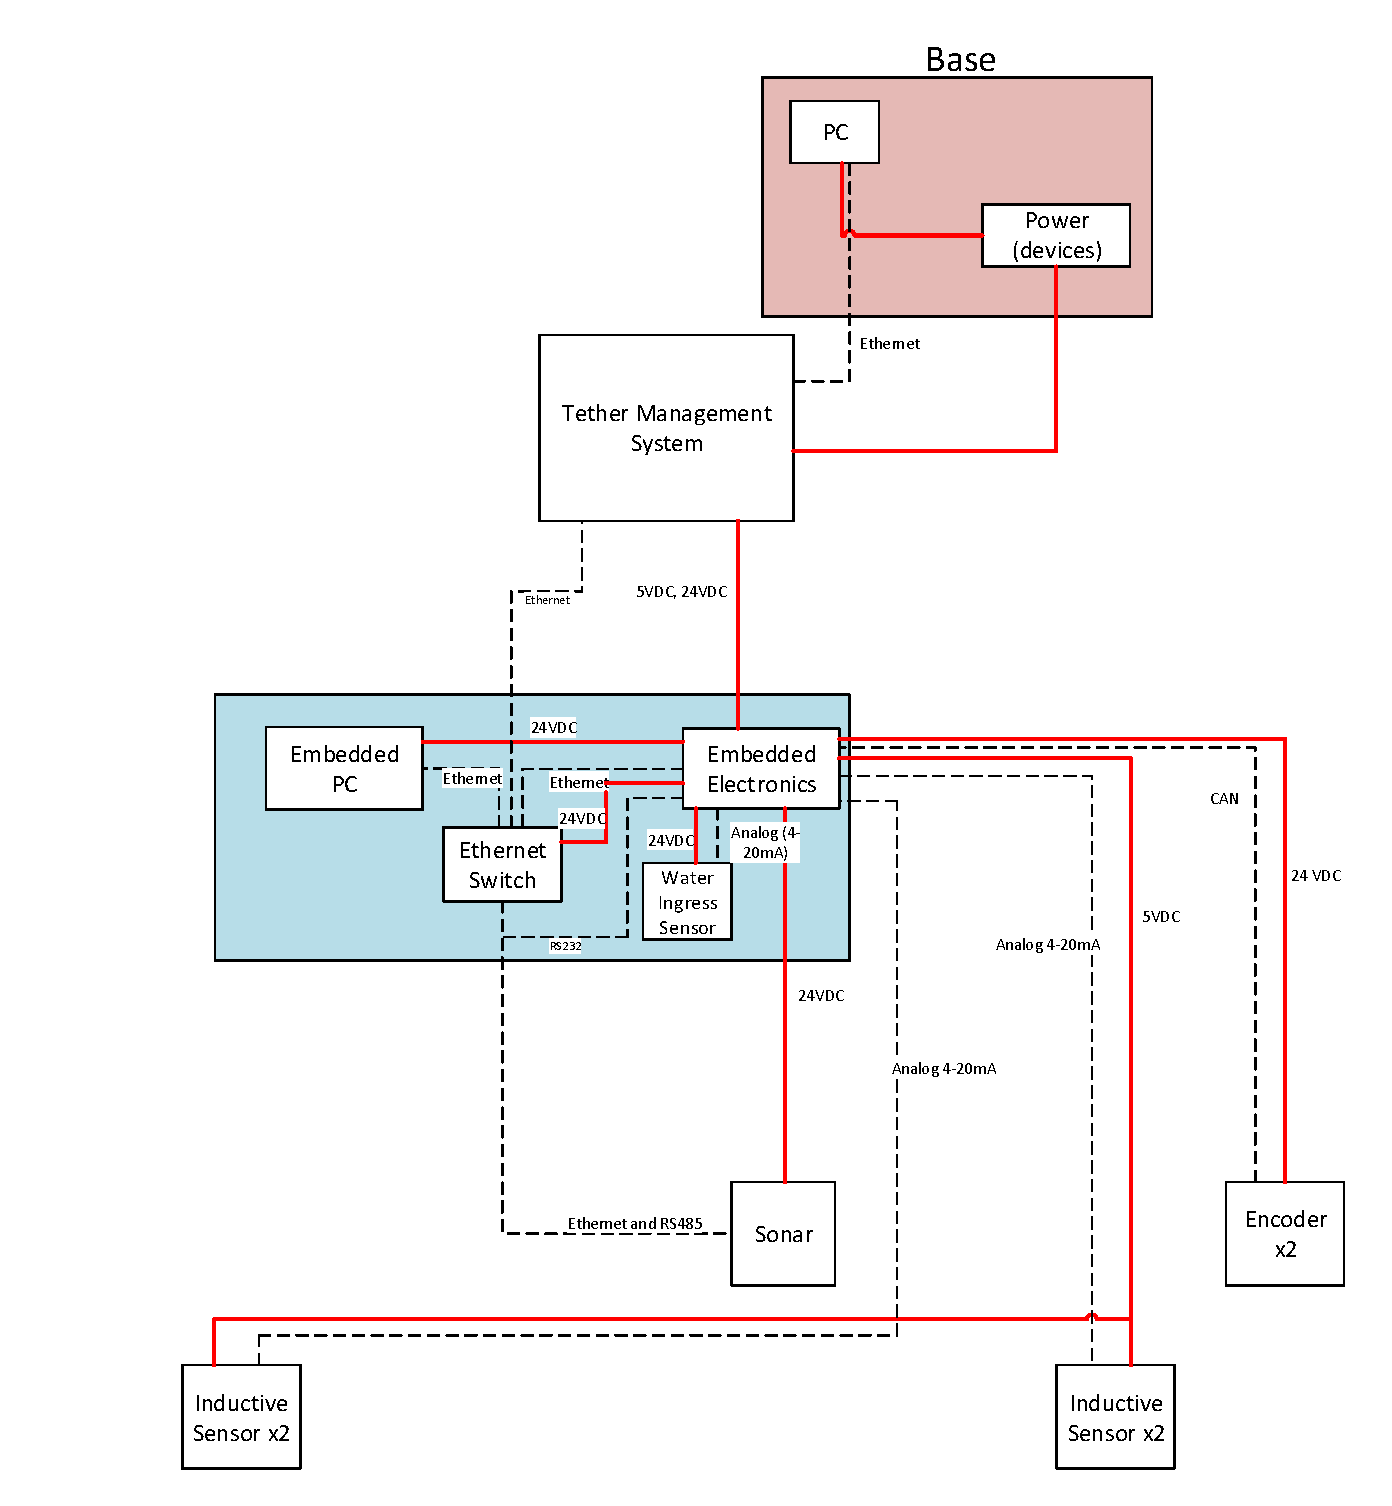
\includegraphics[width=1\columnwidth]{figs/EE/1.pdf}
    \caption{Diagrama de interfaces}
    \label{EE_1}
\end{figure}

\subsubsection{Umbilical}

Cabo especial  de alta resistência mecânica para operação submersa customizado para transmissão de energia e transmissão de dados. O umbilical fornece conexão de dados entre o sistema eletrônico embarcado e a eletrônica de terra. Além disso, o sistema eletrônico embarcado é alimentado pelo umbilical. A taxa de transmissão mínima necessária para o Umbilical é de 1xRS485 

\subsubsection{Eletrônica de superfície - base}

A eletrônica de superfície na base será composta por

\begin{itemize}
	\item PC Industrial com interface Wi-Fi
	\item 230V de entrada de alimentação 
	\item interfaces USB e LAN para periféricos 
	\item Caixa Pelicase para a eletrônica
\end{itemize}

A fonte irá transmitir a potência necessária a todo o sistema embarcado
através do umbilical.

O PC processará todos os dados recebidos do sistema embarco e publicará na
internet ou disponibilizará através do WiFi.

\subsubsection{Eletrônica de superfície - remota}
O operador poderá monitorar todos os sensores através de um tablet com sistema
de rede WiFi. 

\subsubsection{Carretel}
O carretel industrial é necessário ao menos para fornecer alimentação para a
bomba e comunicação para o sonar durante as operações que envolvam limpeza de
sedimentos.
 
Devido à necessidade de montagem mecânica e ao fato deste estar vinculado ao
guindaste e não ao \textit{Lifting Beam}, deve preferencialmente ser utilizado
somente um carretel, de forma a simplificar a montagem mecânica do sistema e se
intervir ao mínimo no guindaste em si. Por esse mesmo motivo, deve ser utilizado
um carretel de perfil compacto.
 
A definição do carretel a ser utilizado está condicionada às características do
sistema de potência. A especificação elétrica da bomba e o cabeamento necessário
para alimentá-la é fundamental para definir as características do elemento. O
peso das blindagens necessárias para o cabeamento da bomba e do par trançado
para comunicação também devem ser considerados.

\subsection{Operação Excepcional 1 - Inspeção}
\label{sis:sol:1}
A utilização de mergulhadores para a realização da operação de inspeção, além de
perigosa, é ineficiente, já que a visibilidade do Rio Madeira é muito
comprometida devido a sedimentos em suspensão no rio. A solução proposta
consiste em realizar a inspeção por meio de um sonar, que irá mapear a a
superfície a ser inspecionada afim de encontrar objetos estranhos e/ou a causa
da falha nas operações de inserção e remoção.

O sonar será acoplado ao \emph{Lifting Beam}, de maneira que a inspeção possa
ser realizada através da operação do guindaste, similarmente à operação de
inserção ou remoção de um \emph{stoplog}. Não haverá a necessidade de nenhuma
alteração estrutural tanto no Lifting Beam, quanto no guindaste, não violando,
assim, nenhum tipo de garantia do equipamento.

A reconstrução da superfície analisada será exibida para o operador do
guindaste, assim como no \emph{tablet} em terra. A visualização possibilitará,
então, a identificação de objetos estranhos e a possível causa do problema.

\subsection{Operação Excepcional 2 - Remoção de sedimentos sobre o olhal}

A remoção de sedimentos do \emph{olhal} que poderiam vir a dificultar ou impedir
um engate de sucesso da \emph{garra pescadora} (subseção \ref{op:rem:2}) será
feito atráves de uma bomba submarina. Esta sendo acoplada ao \emph{Lifting
Beam} com uma posição e ângulo determinados é capaz de eficientemente remover os
pequenos detritos que impediriam a passagem da \emph{garra pescadora} pelo
\emph{olhal} e podendo ser comandado remotamente.
